\chapter{Chip Characterization}

After the chip was fabricated, characterizations were done on each sensor site to determine the best shape, size, pitch, and organization of the electrodes. There are 21 sensor sites on the chip. Each sensor site has four working-electrode areas. Each area has either one or two working electrodes, depending on if it is a 3- or 4-electrode system, respectively.

\section{Sensor Site Characterization}

The 21 sensor sites were characterized to find the best general electrode construction. This was done using differential pulse voltammetry (DPV). DPV is a technique similar to cyclic voltammetry (CV), but which is better because [TODO]. A CH Instruments 660B potentiostat was used to perform all of the following tests. Tests were performed on a probestation (Figure \ref{probestation}) by attaching a PDMS well to prevent solutions from leaking onte probe pads (Figure \ref{chip-top}), then lowering pins onto the probe pads of the chip (Figure \ref{chippins}, \ref{chippins-top}), which were connected to the reference, auxilliary, and working electrode leads of the potentiostat (Figure \ref{potentiostatleads}).

\begin{figure}
	\centering
	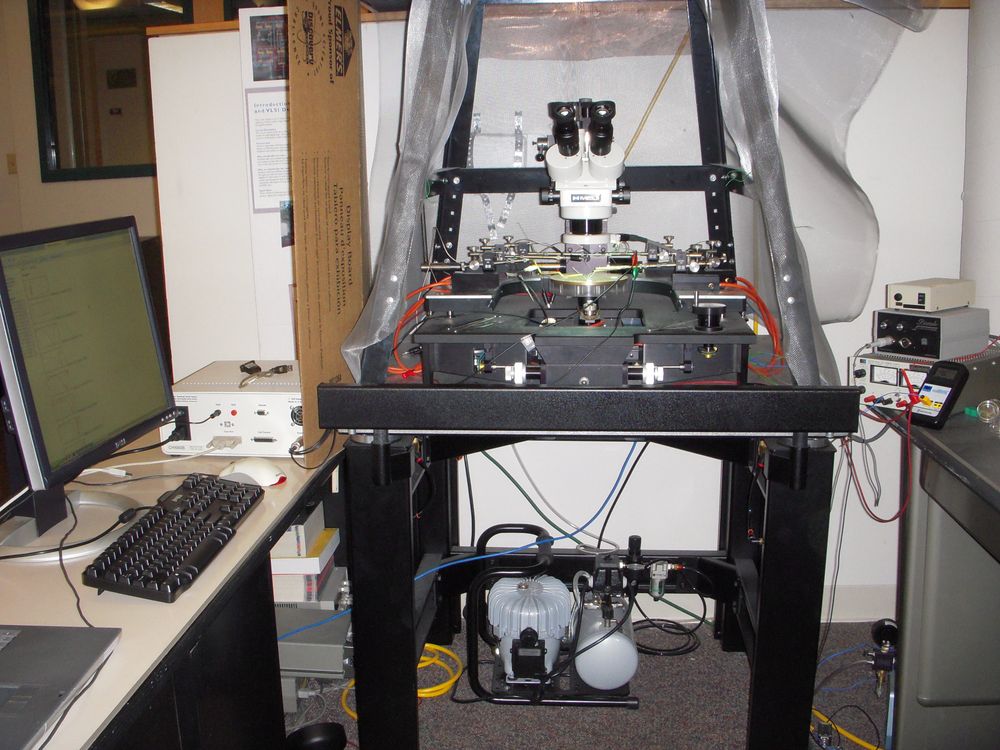
\includegraphics[width=\linewidth]{figures/probestation.png}
	\caption[Probestation.]{Probestation enclosed in a Faraday cage, and connected to the potentiostat.}
	\label{probestation}
\end{figure}

\begin{figure}
	\centering
	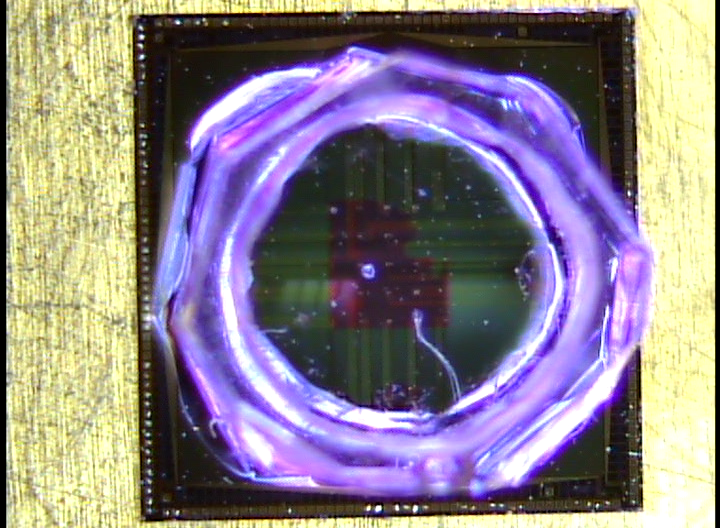
\includegraphics[width=\linewidth]{figures/chip-top.png}
	\caption{Chip with PDMS well attached.}
	\label{chip-top}
\end{figure}

\begin{figure}
	\centering
	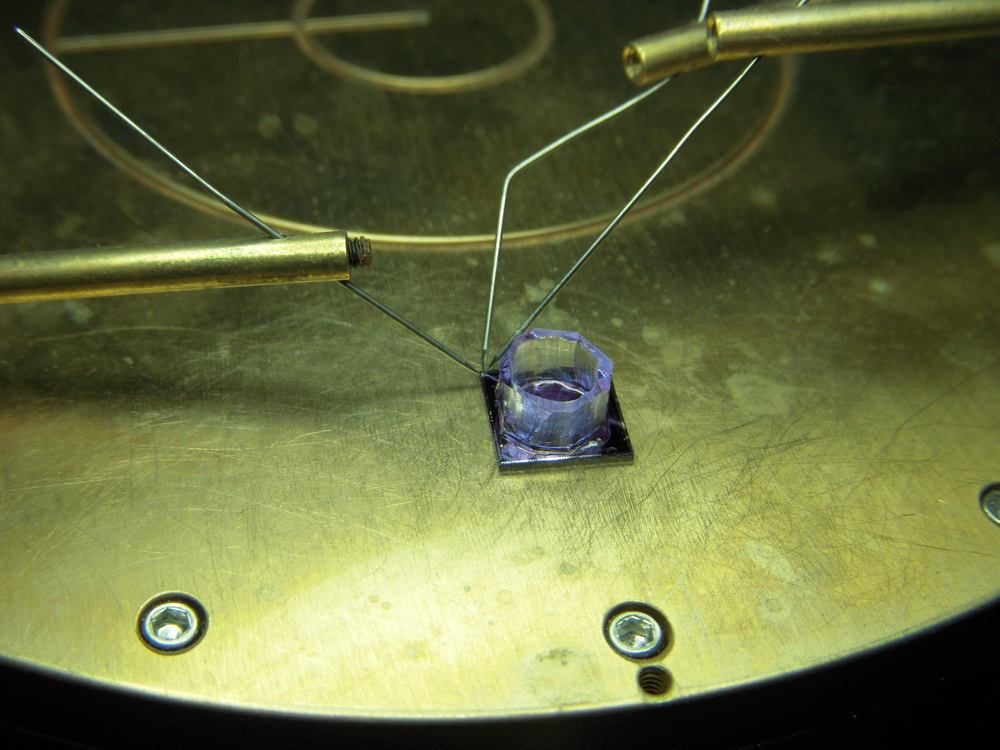
\includegraphics[width=\linewidth]{figures/chippins.png}
	\caption{Pins lowered onto probe pads of the chip.}
	\label{chippins}
\end{figure}

\begin{figure}
	\centering
	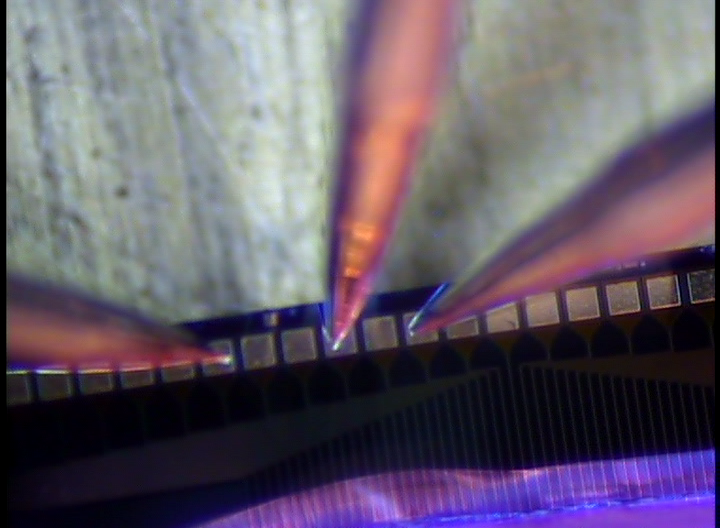
\includegraphics[width=\linewidth]{figures/chippins-top.png}
	\caption{Pins lowered onto probe pads of the chip, top view.}
	\label{chippins-top}
\end{figure}

\begin{figure}
	\centering
	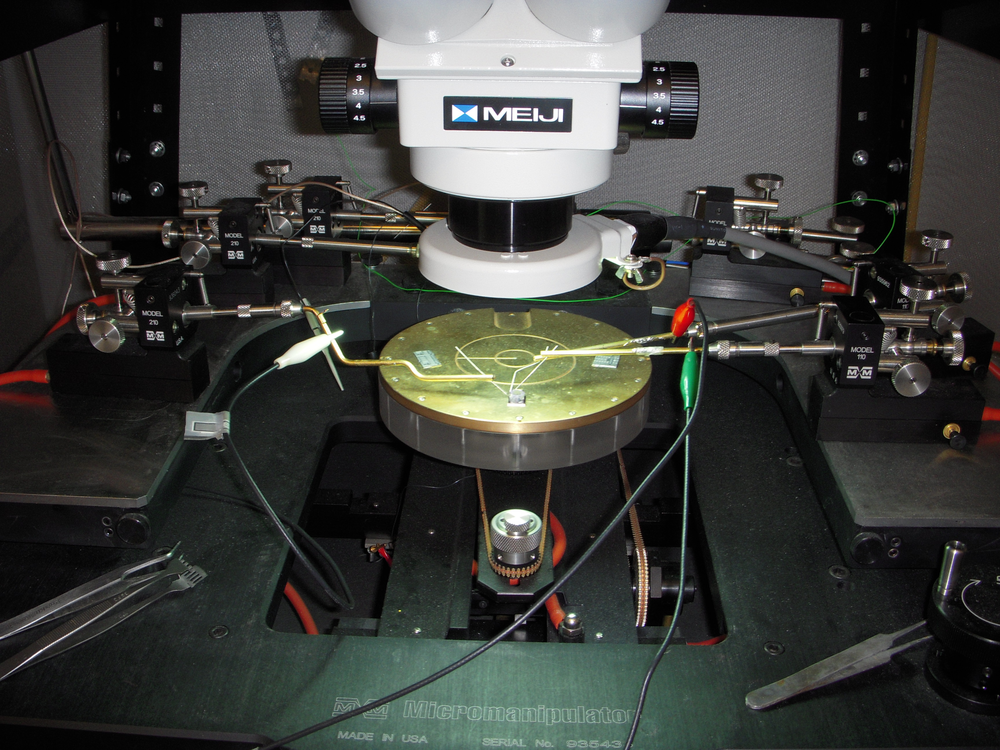
\includegraphics[width=\linewidth]{figures/potentiostatleads.png}
	\caption[Potentiostat leads connected to pins.]{Potentiostat leads for reference, auxilliary, and working electrodes connected to chip pins (white, red, and green, respectively).}
	\label{potentiostatleads}
\end{figure}

The method used was to test two random sensors on each of the 21 sensor sites with 3 tests on each sensor, thus 6 tests on each sensor site. A cleaning was done on each sensor before testing using CV from 1.0V to -0.3V at 1V/s and 20 cycles with $\mathrm{H_2SO_4}$. Tests were performed with DPV from -0.2V to 0.2V with 0.3mM norepinephrine in 0.1M $\mathrm{H_2SO_4}$. A peak formed at around 0.0V. The amplitude of the highest part of the peak in relation to the average baseline (the straight line between the beginning and end of the peak) was taken as the value of a test. Results were compiled by averaging all six tests from each sensor site (Table \ref{DPV results}).

\begin{table}
	\begin{tabular}{lll}
		Sensor & \% of max & Avg. value \\
		\hline
		17 & 100.0 $\pm$ 4.0 & 7.04e-10 $\pm$ 2.83e-11 \\
		8 & 77.9 $\pm$ 5.5 & 5.48e-10 $\pm$ 3.85e-11 \\
		16 & 75.7 $\pm$ 1.8 & 5.32e-10 $\pm$ 1.28e-11 \\
		7 & 71.5 $\pm$ 3.0 & 5.03e-10 $\pm$ 2.13e-11 \\
		18 & 58.8 $\pm$ 2.5 & 4.14e-10 $\pm$ 1.73e-11 \\
		6 & 57.6 $\pm$ 4.0 & 4.05e-10 $\pm$ 2.79e-11 \\
		15 & 55.2 $\pm$ 3.5 & 3.89e-10 $\pm$ 2.43e-11 \\
		14 & 50.8 $\pm$ 2.1 & 3.57e-10 $\pm$ 1.46e-11 \\
		10 & 47.6 $\pm$ 3.6 & 3.35e-10 $\pm$ 2.50e-11 \\
		5 & 43.0 $\pm$ 1.2 & 3.03e-10 $\pm$ 8.27e-12 \\
		1 & 36.7 $\pm$ 3.5 & 2.58e-10 $\pm$ 2.46e-11 \\
		20 & 26.1 $\pm$ 1.0 & 1.84e-10 $\pm$ 7.29e-12 \\
		0 & 23.8 $\pm$ 5.0 & 1.68e-10 $\pm$ 3.55e-11 \\
		19 & 21.9 $\pm$ 2.0 & 1.54e-10 $\pm$ 1.44e-11 \\
		12 & 19.5 $\pm$ 1.5 & 1.37e-10 $\pm$ 1.05e-11 \\
		4 & 19.2 $\pm$ 1.8 & 1.35e-10 $\pm$ 1.28e-11 \\
		13 & 19.1 $\pm$ 1.0 & 1.34e-10 $\pm$ 7.37e-12 \\
		2 & 17.6 $\pm$ 2.1 & 1.24e-10 $\pm$ 1.49e-11 \\
		9 & 17.5 $\pm$ 0.4 & 1.23e-10 $\pm$ 2.83e-12 \\
		11 & 14.4 $\pm$ 1.9 & 1.01e-10 $\pm$ 1.33e-11 \\
		3 & 11.3 $\pm$ 1.3 & 7.93e-11 $\pm$ 9.48e-12
	\end{tabular}
	\caption[DPV results for sensor sites.]{DPV results for sensor sites sorted by decreasing value.}
	\label{DPV results}
\end{table}

\section{Limit of Detection}

Sensor sites 17 and 8 had the best results. Since those sensors have different electrode configuration [TODO: discuss electrode configuration, shape, etc.], testing was done on both sensors to determine the lowest detectable concentration using the same DPV procedure as above, but with decreasing concentrations of norepinephrine starting at 0.3mM and decreasing by a factor of 3 each iteration (Figure \ref{limit figure}). Sensor 17 (Table \ref{limit 17}) was able to detect down to about 3$\mu$M with a linear fit of $A = 1.88996e-6 * M - 2.36855e-12$, where $A$ is the resulting current in amperes and $M$ is the concentration molarity. Sensor 8 (Table \ref{limit 8}) was able to detect down to about 10$\mu$M with a linear fit of $A = 8.29117e-7 * M + 4.3417e-11$, where $A$ is the resulting current in amperes and $M$ is the concentration molarity.

\begin{table}
	\begin{tabular}{ll}
		Concentration (M) & Peak value \\
		\hline
		0.0003 & 5.609E-10 \\
		0.0003 & 5.591E-10 \\
		0.0001 & 1.988E-10 \\
		0.0001 & 2.082E-10 \\
		0.000033 & 5.701E-11 \\
		0.000033 & 4.788E-11 \\
		0.000011 & 1.306E-11 \\
		0.000011 & 1.439E-11 \\
	\end{tabular}
	\caption[Detection limit results for sensor 17.]{Detection limit results for sensor 17 sorted by decreasing concentration.}
	\label{limit 17}
\end{table}

\begin{table}
	\begin{tabular}{ll}
		Concentration (M) & Peak value \\
		\hline
		0.0003 & 2.926E-10 \\
		0.0003 & 2.663E-10 \\
		0.0001 & 1.786E-10 \\
		0.0001 & 1.753E-10 \\
		0.000033 & 3.276E-11 \\
		0.000033 & 3.296E-11 \\
	\end{tabular}
	\caption[Detection limit results for sensor 8.]{Detection limit results for sensor 8 sorted by decreasing concentration.}
	\label{limit 8}
\end{table}

\begin{figure}
	\centering
	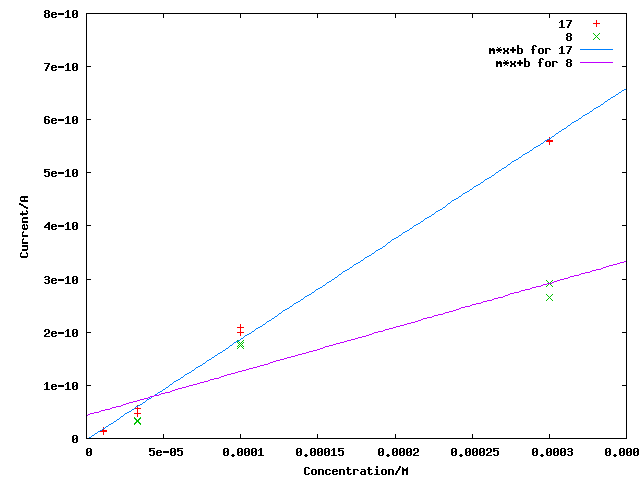
\includegraphics[width=\linewidth]{figures/limit.png}
	\caption{Detection limits.}
	\label{limit figure}
\end{figure}

\section{Electrode Orientation}

In addition to the characterizations above, DPV tests were done to compare working-electrode areas within one sensor site, and auxilliary and reference electrode configurations. Each sensor site contains four working-electrode areas. There are four types of working-electrode configurations and four types of sensor site configurations. The working electrodes are either a 3-electrode system or a 4-electrode system. There is one type of 3-electrode system. There are three types of 4-electrode systems, which will be called ``C'' (Figure \ref{4-C}), ``inverse C'' (Figure \ref{4-I}), ``and F'' (Figure \ref{4-F}), due to the electrode shapes. Areas of the working electrodes are listed in Table \ref{electrode-area}.

\begin{figure}
	\centering
	
\includegraphics[width=0.3\linewidth]{figures/4-C.png}
	\caption{``C''-type working-electrode pair.}
	\label{4-C}
\end{figure}

\begin{figure}
	\centering
	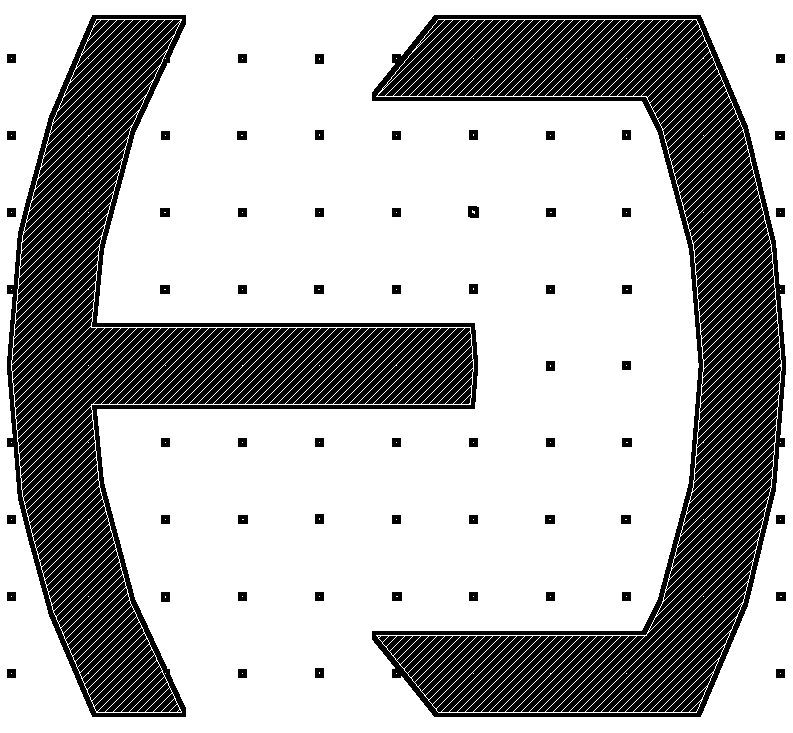
\includegraphics[width=0.3\linewidth]{figures/4-I.png}
	\caption{``Inverse C''-type working-electrode pair.}
	\label{4-I}
\end{figure}

\begin{figure}
	\centering
	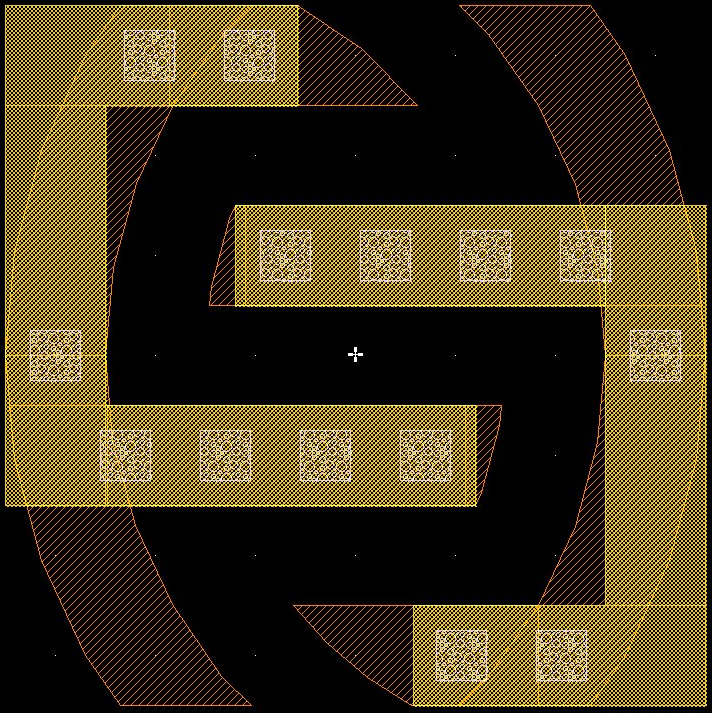
\includegraphics[width=0.3\linewidth]{figures/4-F.png}
	\caption{``F''-type working-electrode pair.}
	\label{4-F}
\end{figure}

\begin{table}
	\begin{tabular}{l|l|l}
		\textbf{electrode system} & \textbf{areas} & \textbf{perimiters} \\
		\hline
		3 & 1, 2.25, 4, 4 & 4, 6, 8, 8 \\
		4, ``C'' & 10.885, 11.342 & 24.700, 25.081 \\
		4, ``inverse C'' & 14.267, 15.119 & 30.793, 32.835 \\
		4, ``F'' & 21.771, 21.738 & 46.636, 46.796
	\end{tabular}
	\caption[Working-electrode areas and perimiters.]{Working-electrode areas, in $\mu \mathrm{m}^2$, and perimiters, in $\mu \mathrm{m}$. The 3-electrode entry lists the different sizes that are in one sensor site. The two electrodes with an area of 4 have different spacings [TODO: define spacing]. The 4-electrode entries list the areas of the left and right electrode, respectively. All working-electrode areas within one sensor site are the same for 4-electrode systems.}
	\label{electrode-area}
\end{table}

\begin{table}
	\begin{tabular}{p{4cm}|p{2cm}|p{2cm}|p{2.5cm}|p{2cm}}
		electrode system: & \textbf{3} & \textbf{4, C} & \textbf{4, inverse C} & \textbf{4, F} \\
		\hline
		\textbf{2 auxilliary} & 0, 1, 2, 20 (Figure \ref{s00}) & & & \\
		\hline
		\textbf{common reference, top \& bottom} & 3, 4, 9, 19 (Figure \ref{s03}) & & & \\
		\hline
		\textbf{common reference top, common auxilliary bottom} & & 5 (Figure \ref{s05}) & 6, 7 (Figure \ref{s06}) & 8, 17 (Figure \ref{s17}) \\
		\hline
		\textbf{common reference top, common auxilliary on 3 sides} & 11, 12, 13 (Figure \ref{s11}) & 14, 15 (Figure \ref{s14}) & 10 (Figure \ref{s10}) & 16, 18 (Figure \ref{s16})
	\end{tabular}
	\caption{Sensor site configurations.}
	\label{sensor-config}
\end{table}

\begin{figure}
	\centering
	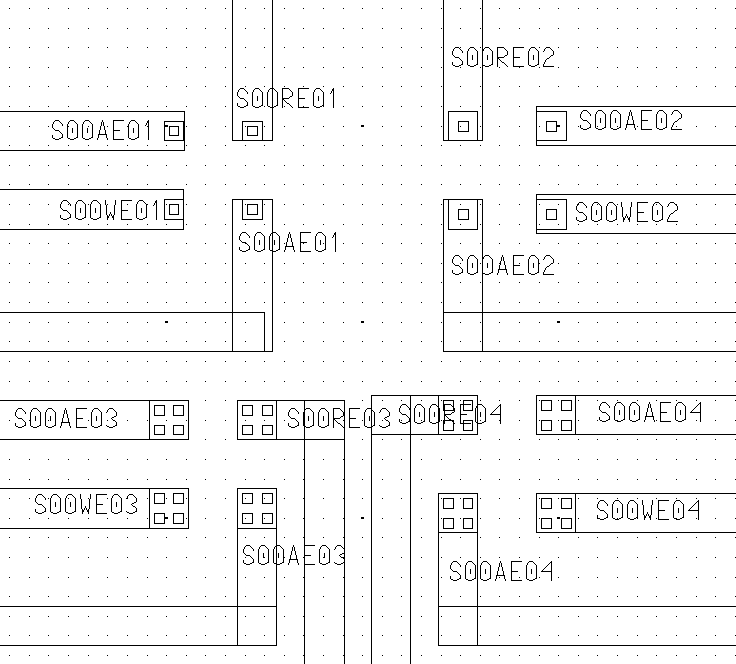
\includegraphics[width=0.7\linewidth]{figures/s00.png}
	\caption{Sensor 0.}
	\label{s00}
\end{figure}

\begin{figure}
	\centering
	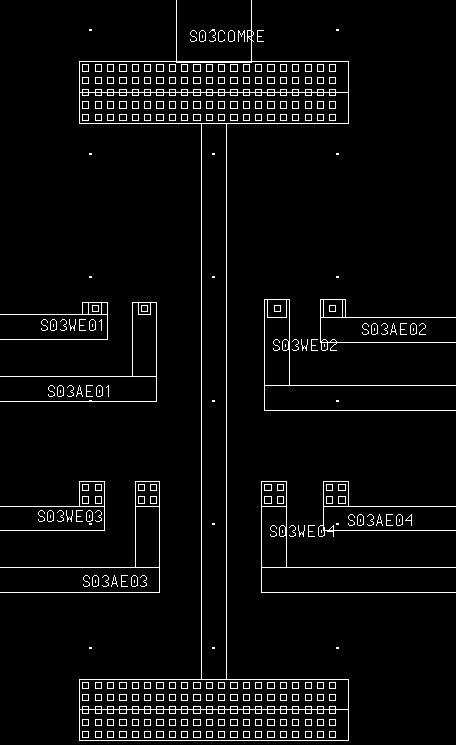
\includegraphics[width=0.7\linewidth]{figures/s03.png}
	\caption{Sensor 3.}
	\label{s03}
\end{figure}

\begin{figure}
	\centering
	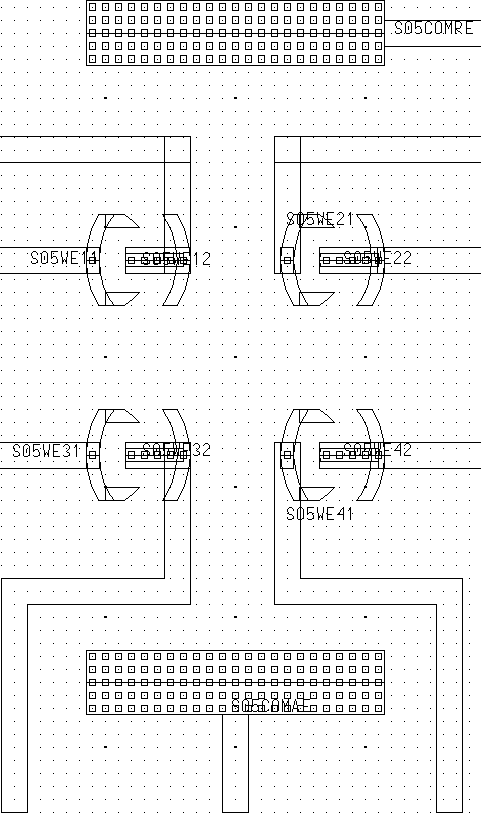
\includegraphics[width=0.7\linewidth]{figures/s05.png}
	\caption{Sensor 5.}
	\label{s05}
\end{figure}

\begin{figure}
	\centering
	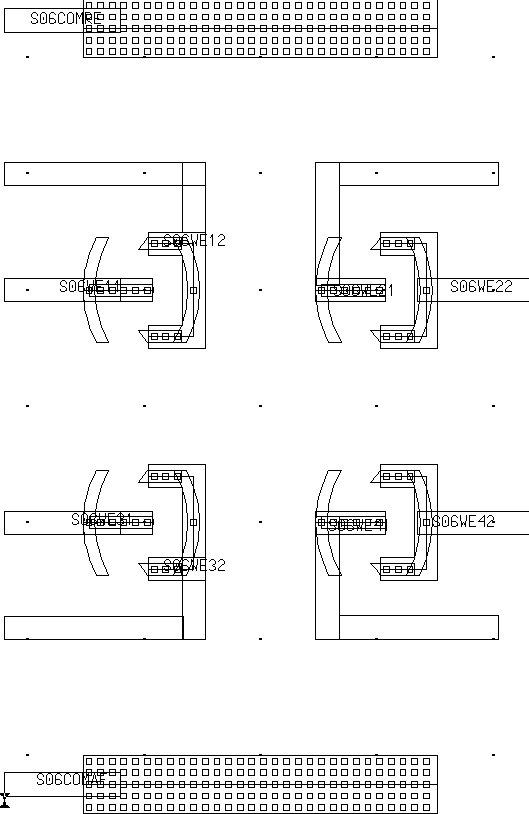
\includegraphics[width=0.7\linewidth]{figures/s06.png}
	\caption{Sensor 6.}
	\label{s06}
\end{figure}

\begin{figure}
	\centering
	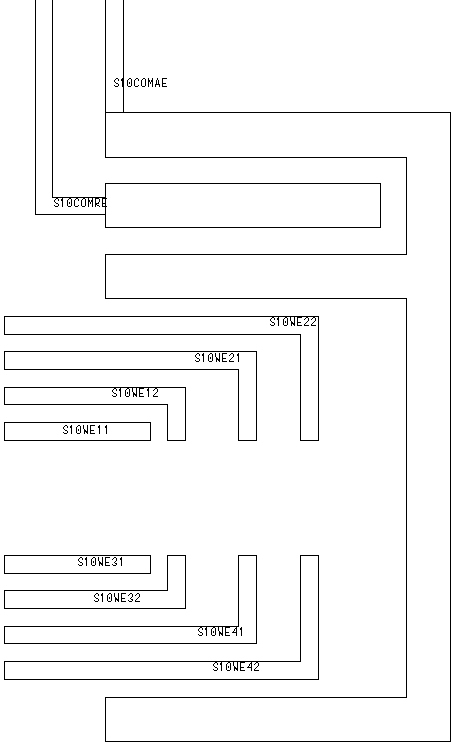
\includegraphics[width=0.7\linewidth]{figures/s10.png}
	\caption{Sensor 10.}
	\label{s10}
\end{figure}

\begin{figure}
	\centering
	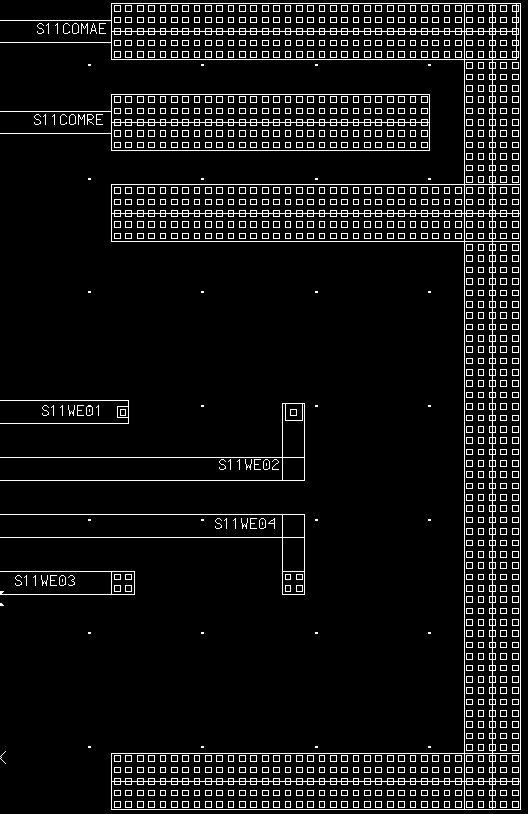
\includegraphics[width=0.7\linewidth]{figures/s11.png}
	\caption{Sensor 11.}
	\label{s11}
\end{figure}

\begin{figure}
	\centering
	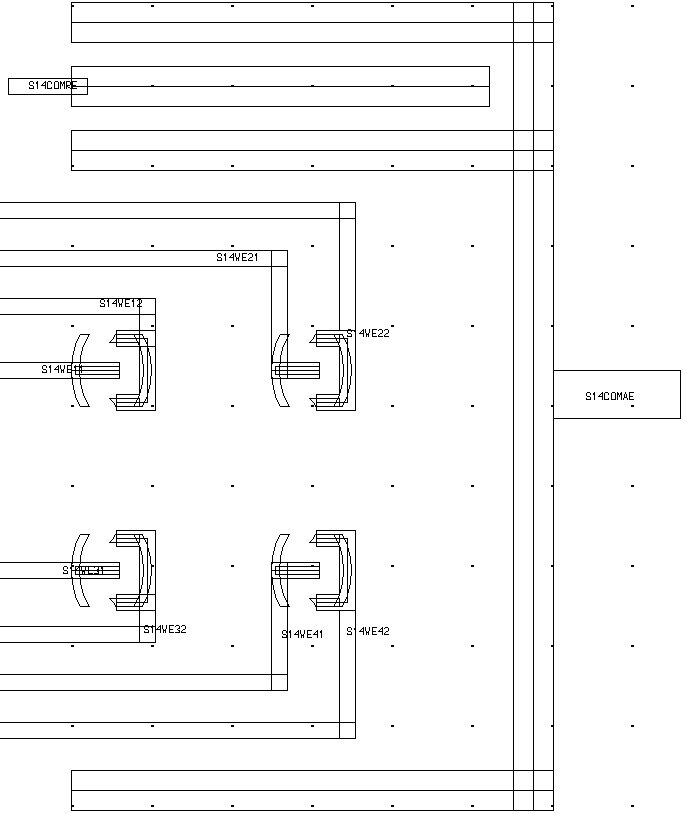
\includegraphics[width=0.7\linewidth]{figures/s14.png}
	\caption{Sensor 14.}
	\label{s14}
\end{figure}

\begin{figure}
	\centering
	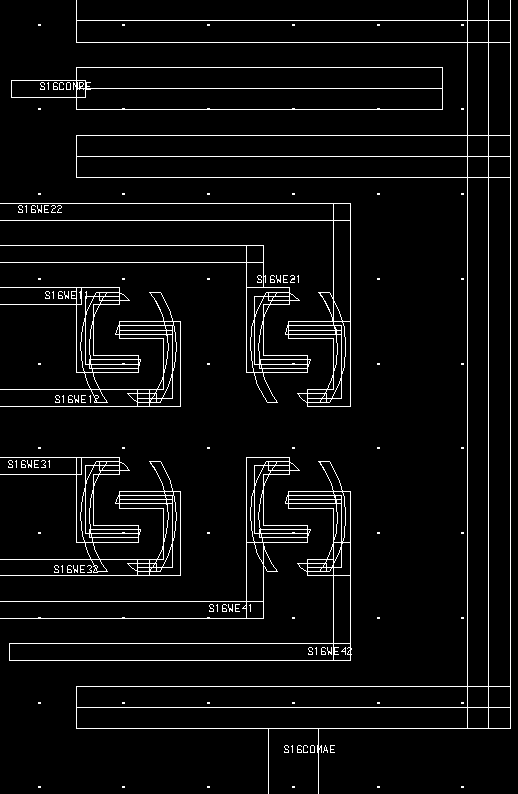
\includegraphics[width=0.7\linewidth]{figures/s16.png}
	\caption{Sensor 16.}
	\label{s16}
\end{figure}

\begin{figure}
	\centering
	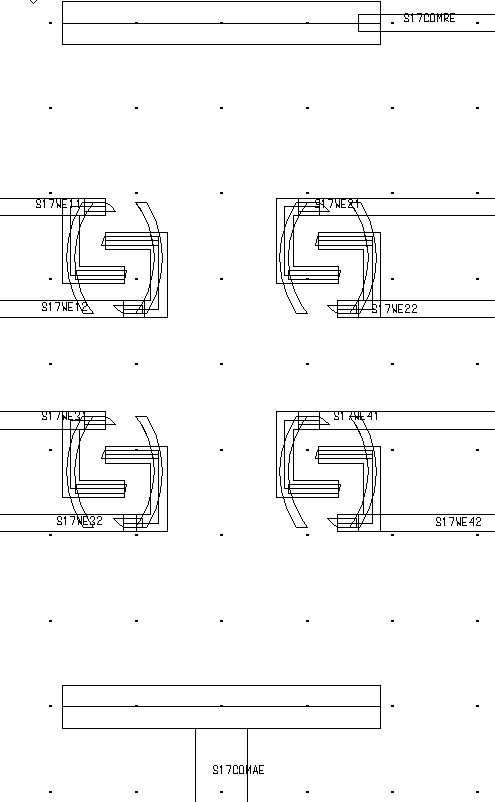
\includegraphics[width=0.7\linewidth]{figures/s17.png}
	\caption{Sensor 17.}
	\label{s17}
\end{figure}

To test the importance of the position of a working electrode (e.g., its relative position to the auxilliary and reference electrodes), the standard DPV tests were done on multiple working electrodes on sensors 16 (Figure \ref{s16}) and 17 (Figure \ref{s17}), which have identical working-electrode types (4-electrode, type ``F''). Two tests were done on each of working electrodes 12 and 32, and averaged by working electrode (Table \ref{dpv-specific}). The working electrodes closest to the auxilliary electrode both performed better than the two working electrodes furthest from the auxilliary electrode. We conclude that closeness to an auxilliary electrode yields better results than closeness to the reference electrode.

From the same tests we can also conclude that the sensor-site orientation of sensor 17 (common reference on one side, common auxilliary on the other) is better than sensor 16 (common reference on one side, common auxilliary surrounding the working electrodes on three sides).

\begin{table}
	\begin{tabular}{lllllll}
		sensor & electrode & chip 1 & chip 3 & chip 4 & distance & area \\
		\hline
		02 & 01 &           & 1.493e-10 $\pm$ 7.3e-12 & 1.632e-10 $\pm$ 1.6e-12 &  3.00 & 1 \\
		02 & 02 &           & 1.921e-10 $\pm$ 4.1e-12 & 2.120e-10 $\pm$ 8.9e-12 &  3.00 & 2.25 \\
		02 & 03 &           & 1.940e-10 $\pm$ 1.1e-11 & 2.250e-10 $\pm$ 2.0e-12 &  2.50 & 4 \\
		02 & 04 &           & 1.419e-10 $\pm$ 8.5e-12 & 1.850e-10 $\pm$ 4.6e-12 &  3.00 & 4 \\
		07 & 12 & 5.169e-10 & 4.774e-10 $\pm$ 2.1e-11 & 4.994e-10 $\pm$ 1.2e-11 & 45.48 & 15.119 \\
		07 & 32 & 3.245e-10 & 4.963e-10 $\pm$ 1.1e-11 & 4.072e-10 $\pm$ 2.2e-12 & 20.40 & 15.119 \\
		16 & 12 & 5.157e-10 & 7.212e-10 $\pm$ 2.4e-11 & 6.188e-10 $\pm$ 1.3e-11 & 13.50 & 21.738 \\
		16 & 32 & 6.494e-10 & 6.349e-10 $\pm$ 5.2e-12 & 6.989e-10 $\pm$ 1.0e-11 & 13.50 & 21.738 \\
		17 & 11 & 6.562e-10 &                         &                         & 43.47 & 21.771 \\
		17 & 12 & 4.949e-10 & 5.533e-10 $\pm$ 8.5e-12 & 6.420e-10 $\pm$ 9.2e-12 & 43.47 & 21.738 \\
		17 & 31 & 6.913e-10 &                         &                         & 18.46 & 21.771 \\
		17 & 32 & 6.593e-10 & 6.360e-10 $\pm$ 5.9e-12 & 6.284e-10 $\pm$ 1.2e-11 & 18.46 & 21.738 \\
		18 & 12 & 5.570e-10 & 5.377e-10 $\pm$ 8.8e-12 & 6.130e-10 $\pm$ 8.5e-12 & 18.50 & 21.738 \\
		18 & 32 & 5.683e-10 &                         & 4.965e-10 $\pm$ 2.8e-12 & 18.50 & 21.738

	\end{tabular}
	\caption[Results of further DPV tests on specific working electrodes.]{Results of further DPV tests on specific working electrodes. Outputs are given from averaged data from runs on chips 1, 3, and 4 with standard error in amperes. The distance column lists the distance of the working to the auxilliary electrode from Table \ref{electrode distance} in $\mu \mathrm{m}$. The area column lists the area of the working electrode from Table \ref{electrode-area} in $\mu \mathrm{m}^2$. Chip 2 was not performing well and was skipped. Chips 3 and 4 used the same solution. Chip 1 used a separate solution. They were both mixed to be identical, but at concentrations this low, that is difficult to guarantee. Thus, do not use these data without adjusting for relative performance.}
	\label{dpv-specific}
\end{table}

\begin{table}
	\begin{tabular}{llll}
		sensor & electrode from & electrode to & distance ($\mu \mathrm{m}$) \\
		\hline
		0 & *01 & *01 & 3.00 \\
		0 & *02 & *02 & 3.00 \\
		0 & *03 & *03 & 2.50 \\
		0 & *04 & *04 & 3.00 \\
		\multicolumn{4}{l}{sensor 0 is the same as sensor 1, 2} \\
		3 & we01 & ae01 & 3.00 \\
		3 & we02 & ae02 & 3.00 \\
		3 & we03 & ae03 & 2.50 \\
		3 & we04 & ae04 & 3.00 \\
		\multicolumn{4}{l}{sensor 3 is the same as sensor 4, 9} \\
		5 & we1*, we2* & comae & 26.55 \\
		5 & we3*, we4* & comae & 11.51 \\
		6 & we1*, we2* & comae & 35.54 \\
		6 & we3*, we4* & comae & 15.51 \\
		7 & we1*, we2* & comae & 45.48 \\
		7 & we3*, we4* & comae & 20.40 \\
		8 & we1*, we2* & comae & 33.53 \\
		8 & we3*, we4* & comae & 13.53 \\
		10 & we* & comae & 11.5 \\
		11 & we01 & comae & 14.47 \\
		11 & we02 & comae & 14.24 \\
		11 & we03, we04 & comae & 13.96 \\
		12 & we01 & comae & 19.50 \\
		12 & we02 & comae & 19.21 \\
		12 & we03, we04 & comae & 18.98 \\
		13 & we01 & comae & 24.53 \\
		13 & we02 & comae & 24.26 \\
		13 & we03, we04 & comae & 24.05 \\
		14 & we* & comae & 20.50 \\
		15 & we* & comae & 15.50 \\
		16 & we* & comae & 13.50 \\
		17 & we1*, we2* & comae & 43.47 \\
		17 & we3*, we4* & comae & 18.46 \\
		18 & we* & comae & 18.50 \\
		19 & we01 & ae01 & 2.00 \\
		19 & we02 & ae02 & 3.00 \\
		19 & we03 & ae03 & 2.50 \\
		19 & we04 & ae04 & 3.00 \\
		\multicolumn{4}{l}{sensor 19 is the same as sensor 20}
	\end{tabular}
	\caption[Electrode distances.]{Electrode distances, measured by the two closest edges. ``we'' means working electrode; ``ae'' means auxilliary electrode; ``re'' means reference electrode. ``com'' means common. For example, comae means common auxilliary electrode. A * means all electrodes that fit the rest of the expression. For example, *01 means we01, ae01, re01.}
	\label{electrode distance}
\end{table}
